
\documentclass{article}

\usepackage{lipsum}
\usepackage[margin=1in,includefoot]{geometry}
\usepackage{graphicx}
\usepackage{float}
\usepackage[hidelinks]{hyperref}
\usepackage{amsmath}
\usepackage{amssymb}
\usepackage{color}


\usepackage[usenames,dvipsnames]{xcolor}
\usepackage{listings}







% Header and Footer Stuff
\usepackage{fancyhdr}
\pagestyle{fancy}
\fancyhead{}
\fancyfoot{}
\fancyfoot[R]{\thepage}
\renewcommand{\headrulewidth}{0pt}
\renewcommand{\footrulewidth}{0pt}


\definecolor{dkgreen}{rgb}{0,0.6,0}
\definecolor{gray}{rgb}{0.5,0.5,0.5}
\definecolor{mauve}{rgb}{0.58,0,0.82}

\lstset{
  language=VHDL,
  aboveskip=3mm,
  belowskip=3mm,
  showstringspaces=false,
  columns=flexible,
  basicstyle={\small\ttfamily},
  numbers=none,
  numberstyle=\tiny\color{gray},
  keywordstyle=\color{blue},
  commentstyle=\color{dkgreen},
  stringstyle=\color{mauve},
  breaklines=true,
  breakatwhitespace=true,
  tabsize=3
}












\begin{document}

\begin{titlepage}
	#include <iostream>
#include <unistd.h>
#include <cstdlib>
#include <cstring>
#include <netdb.h>
#include <stdio.h>
#include <sys/socket.h>
#include <arpa/inet.h>
#include <algorithm>
#include <stdlib.h>
#include <string.h>
#include <bitset>
#include <sstream>
#include <unistd.h>
#include <netinet/in.h>
#include <cerrno>
#include <cstring>
#include <fstream>
#include <time.h>
#include <sys/uio.h>
#include <zlib.h>

#define BUFLEN 1024
#define PORT 5562
using namespace std;
static const string compar="011111";

/*8 bytes*/
/*2 bytes for header - sequence number*/
/*4 bytes for packet*/
/*2 bytes for trailer - crc*/ 


/* alorithm of calculating the 'checksum'*/
 /* polynomial*/

/* converts int from binary text*/


/*******************************************************/
    	/*CRC*/
/*******************************************************/
int getIntFromBinaryText(const char* text)
{
    int value = 0;
    while(*text)
    {
        value <<= 1;
             if(*text == '1')
             {   
              	value |= 1;
              }
        else if(*text == '0');          
        else                     
        	return -1; /* invalid input*/
        	/*return a negative number to indicate error*/
        ++text;
    }
 
    return value;
}
/*converts the text back to binary string*/
std::string getBinaryTextFromInt(int value)
{
    std::string text;
    
 	/*assume unsigned*/
    while(value > 0)
    {
        if(value & 1)       
        {
        	text += '1';
        }
        else                
        {
        	text += '0';
        }
        value >>= 1;
    }
 
    if(text.empty())        
    {
    	return "0";
    }
    std::reverse( text.begin(), text.end() );       
    return text;
}
/*******************************************************/

/*counts bytes in a file*/
long GetFileSize(const char* filename)
{
    long size;
    FILE *f;
 /*opened in a binary format */
 /*r to read*/
 /*b to open in binary*/
    f = fopen(filename, "rb");
    if (f == NULL)
    {
    	return -1;
    }
    fseek(f, 0, SEEK_END);
    size = ftell(f);
    fclose(f);
 
    return size;
}


/*Alphanumeric Random Character Generator*/
int RandGen()  
{
	int num = 0;
	// random sub-range*/
	num = rand()%3;  
 	//range0: numeric*/
	if (num == 0)      
	{
		return (rand()%10)+48;
	}   
	// range1: upper characters
	if (num == 1)       
	{
		return (rand()%26)+65;
	}
	// range2: lower characters
	if (num == 2)        
	{
		return (rand()%26)+97;
	}
}

bool bitsize(string const &tmp, string const &compar)
{
	return tmp.size() >=compar.size() && tmp.compare(tmp.size() - compar.size(), compar.size(), compar)==0;
}


void server_main()
{	
	cout<<"***************************************"<<endl;
	cout<<"***************UDP_SERVER**************"<<endl;
	cout<<"***************************************"<<endl;
	int sock;
	struct sockaddr_in server_socket;
	struct sockaddr_in client_socket;
	
	int one=1;
	long filesize;
	// declare the 'out' stream
	ofstream out;    
	filesize  = GetFileSize("test.txt");
	
	std::ofstream ofs;
	ofs.open("out.txt", std::ofstream::out | std::ofstream::trunc);
	ofs.close();
	
	
	/*******************************************************/
    	/*SOCKET CREATION*/
    	/*******************************************************/
	/*Define socket as UDP*/
	if ((sock = socket(PF_INET, SOCK_DGRAM, IPPROTO_UDP)) < 0)exit(0);
	setsockopt(sock, SOL_SOCKET, SO_REUSEPORT, &one, sizeof(one));
	/*clear memory*/
	memset(&server_socket, 0, sizeof(server_socket));
	/*socket family*/
	server_socket.sin_family = AF_INET;
	/*ip adress*/
	server_socket.sin_addr.s_addr = htonl(INADDR_ANY);
	/*port*/
	server_socket.sin_port = htons(PORT);
	
	if (bind(sock, (struct sockaddr *) &server_socket, sizeof(server_socket)) < 0)
		exit(0);
	/*******************************************************/
	char buffer[BUFLEN];
	int received;
	int servHeader1=1;
	int servHeader2=1;
	while (1) 
	{	
	/*******************************************************/
		/*Receives test.txt contents from the client */
	/*******************************************************/
		for(int i=1;i<=filesize/4;i+=4)
		{
			socklen_t client_len = sizeof(client_socket);
			if ((received = recvfrom(sock, buffer, 255, 0, (struct sockaddr *) &client_socket, &client_len)) < 0) 
			{
				exit(0);
			}
			buffer[received] = '\0';
			cout <<"SERVER CONNECTION ON RECEIVING: "<< inet_ntoa(client_socket.sin_addr)<<"\t"<<endl;
			cout<<"SERVER PORT: "<<PORT<<endl;
			cout<<"RECEIVED DATA FRAME: "<<servHeader1<<endl;
			cout <<"RECEIVED DATA SENT FROM CLIENT: "<< buffer<<endl;
			/*converts char to string*/
			string s_buffer(buffer);
			/*unstuff bits*/
  			/*char sa2[s_buffer.length()];
  			s_buffer.copy(sa2, s_buffer.length());
  			string s2one="";
  			string s2two="";
  			/*bitstuffing 
  			for(int i =0 ; i<s_buffer.length();i++)
  			{
  				s2one+= s2two[i];
  				s2two+=s2two[i];
  			
  			
  				if(bitsize(s2one , compar))
  				{
  					s2one ="";
  					i++;
  				}
  			}*/
  			string s2=s_buffer;
			
			cout<<"++++++++++"<<endl;
			string header = s2.substr( 0, 8);
			cout<<"HEADER: "<<header<<endl;
			string packet = s2.substr( 8, 32);
			cout<<"PACKET: "<<packet<<endl;
			string crc = s2.substr(40, 8);
			
			string text=crc;
			int divisor = getIntFromBinaryText("01111111");
			int dividend = getIntFromBinaryText(text.c_str());
  			int remainder = dividend % divisor;
  			string tmp4 = getBinaryTextFromInt(remainder);
  			
  			
  			
  			
  			
  			cout<<"ReCEIVED CRC: "<<crc<<endl;
  			cout<<"CALCULATED CRC: "<<tmp4<<endl;
			cout<<"++++++++++"<<endl<<endl;
			servHeader1++;
			if(crc.compare(tmp4) != 0)
			{
				
				
				cout<<"!!!! DATA NOT  OK !!!!"<<endl<<endl;
			
				cout<<"----------------------"<<endl;
				cout<<"DATA HAS BEEN CORRUPED"<<endl;
				cout<<"RESETTING FRAME INSTANCE"<<endl;
				cout<<"----------------------"<<endl;
				char buffer[BUFLEN]="!!!!";
				socklen_t client_len = sizeof(client_socket);
				if (sendto(sock, buffer, strlen(buffer), 0, (struct sockaddr *) &client_socket, sizeof(client_socket)) < 0)
				{
					cout<<"error here";
					exit(0);
				}
				buffer[received] = '\0';
				
				servHeader1--;
			}
			else
			{
				cout<<"+++ DATA OK +++"<<endl;
				sleep(2);
				
				/***
				bitstuffing happens here
				*/

				if (sendto(sock, buffer, strlen(buffer), 0, (struct sockaddr *) &client_socket, sizeof(client_socket)) < 0)
				{
					cout<<"error here";
					exit(0);
				}
				cout <<"SERVER CONNECTION ON SENDING: "<< inet_ntoa(client_socket.sin_addr)<<"\t"<<endl;
				cout<<"SERVER PORT: "<<PORT<<endl;
				cout<<"RESEND DATA FRAME: "<<servHeader2<<endl;
				cout <<"RESEND DATA SENT FROM CLIENT: "<< buffer<<endl;
				cout<<"-------------"<<endl<<endl<<endl;
				servHeader2++;
				sleep(3);
				
	/*******************************************************/
	/*******************************************************/
		/* open data file*/
    		/*delete contents of file
    		and add new contents*/
    	/*******************************************************/
    				std::ofstream ofs;
				ofs.open("out.txt", std::ofstream::out | std::ofstream::app);
				 
    				std::stringstream sstream(packet);
    				string output;
    				while(sstream.good())
    				{
        				std::bitset<8> bits;
        				sstream >> bits;
        				char c = char(bits.to_ulong());
        				output += c;
    				}
				ofs<<output;
				ofs.close();
				sleep(1);
				
			}
		}
	/*******************************************************/
	}
}

void client_main()
{
	int sock, rc;
	long filesize;
	long begin, end;
	int i = 0;
	int one=1;
	struct sockaddr_in server_socket;
	struct sockaddr_in client_socket;
	/*text file being accessed for proj*/
	ifstream myfile ("test.txt");	
	char crc2char;
	cout<<"***************************************"<<endl;
	cout<<"***************UDP_CLIENT**************"<<endl;
	cout<<"***************************************"<<endl;
	/*****************************************************/
	/*First delete previous contents in file*/
	/*****************************************************/
	// declare the 'out' stream
	ofstream out;    
	// try to open data file
    	out.open("test.txt");  
     	// check if opened
    	if(out.fail())              
    	{ 
		cout << "unable to open test.txt" << endl;
		//return 1; 
    	} 
    	/*delete contents of file*/
    	std::ofstream ofs;
	ofs.open("test.txt", std::ofstream::out | std::ofstream::trunc);
	ofs.close();
	/*******************************************************/
	
	/*******************************************************/
	/* Write 1024 random ASCII characters into file*/
	/*******************************************************/
	/*time the randomness*/
    	srand((unsigned)time(0));
    	/* the loop outputs 1024 
    	alphanumeric characters
    	 into the stream*/
	for(int i = 0;i<1024;i++)   
    	{
	// casting from a number to a character
        	out << static_cast<char>(RandGen());           
    	}
    	out.close();
    	system("---DATA FILE HAS BEEN CREATED---\n");
    	/*******************************************************/
    	
    	/*******************************************************/
    	/*SOCKET CREATION*/
    	/*******************************************************/
	if ((sock = socket(PF_INET, SOCK_DGRAM, IPPROTO_UDP)) < 0)
	{
		exit(0);
	}
	setsockopt(sock, SOL_SOCKET, SO_BROADCAST, &one, sizeof(one));
	/*clear memory*/
	memset(&server_socket, 0, sizeof(server_socket));
	/*socket family*/
	server_socket.sin_family = AF_INET;
	/*Ip adress*/
	server_socket.sin_addr.s_addr = inet_addr("127.0.0.1");
	/*port*/
	server_socket.sin_port = htons(PORT);
	rc= bind(sock, (struct sockaddr *) &client_socket, sizeof(client_socket));
	if (rc < 0) 
	{
		cout<<"Cannot bind port\n";
	}
	/*******************************************************/
	
	
	char buffer[BUFLEN];
	char buf[BUFLEN];
	int num_characters = 0;
	/*while loop to read the number of characters in the file*/
	while (!myfile.eof())
      	{
      	
      		
            myfile.get(buffer[i]);
            i++;
            num_characters ++;
            
      	}  
      	
      	
	filesize  = GetFileSize("test.txt");
      	cout<<"************************"<<endl;
      	cout<<"FILESIZE: "<<filesize <<endl;
      	cout<<"NUMBER OF CHARACTERS: "<<num_characters<<endl;
      	cout<<"************************"<<endl;
      	int frameid=1;
      	int frameid2=1;
      	
      	
        /*******************************************************/
		/*loads .txt into a string */
	/*******************************************************/
      	ifstream ifstrfile("test.txt");
      	string stringfile;
      	ifstrfile.seekg(0, std::ios::end);
      	stringfile.reserve(ifstrfile.tellg());
      	ifstrfile.seekg(0, std::ios::beg);
      	stringfile. assign((istreambuf_iterator<char>(ifstrfile)),istreambuf_iterator<char>());
      	/*******************************************************/
      	
       /*******************************************************/
		/*sends test.txt contents to the server */
	/*******************************************************/
		
	while(1)
	{	
	
		/*splits packet into 4 bits
		thus there will be 256 frames*/
		for(int i=1;i<=filesize/4;i+=4)
		{
			if(i>256)
			{
				cout<<"Protocol Ending";
				exit(0);
			
			}
			
			/*increments through string 
			and copies it to the buffer*/	
			string substr1 = stringfile.substr(i,4);
			string tmp = substr1;
			string tmp2;
			/*127*/
			int divisor = getIntFromBinaryText("01111111");
			string binary_header; 
		
			/*converts the string characters to binary string*/
   			for (std::size_t s = 0; s < tmp.size(); ++s)
  			{
  				/*header conv to binary*/
  				binary_header = std::bitset<8>(frameid).to_string(); 
  				/*packet conv to binary*/
      			 	bitset<8> b(tmp.c_str()[s]);
      			 	tmp2+=b.to_string();
      			 	
  			}
  			
  			
  			string text =tmp2;
  			int dividend = getIntFromBinaryText(text.c_str());
  			int remainder = dividend % divisor;
  			/*crc*/
  			string tmp4 = getBinaryTextFromInt(remainder);
  			/*bitstuffing 
  			char sa[tmp2.length()];
  			tmp4.copy(sa, tmp2.length());
  			string sone="";
  			string stwo="";
  			
  			for(int i =0 ; i<tmp2.length();i++)
  			{
  				sone+= stwo[i];
  				stwo+=stwo[i];
  			
  			
  				if(bitsize(sone , compar))
  				{
  					sone = "";
  					stwo +="0";
  				}
  			}
  			string tmp10=stwo;*/
  			/*tmp3=header+packet*/
  			string tmp3= binary_header+tmp2;
  			/*gremlin*/
  			int v1 = rand() % 4+1;
  			int grm=0;
  			if(v1 <2 )
  			{
  				tmp4 =string ( tmp4.rbegin(), tmp4.rend());
  			grm++;
  			} 
  			
  			
  			/*frame=(header+packet)+crc*/
  			string tmp5 = tmp3+tmp4;
  			/*coppies binary string to char array*/
			strcpy(buffer,tmp5.c_str());
			
			if (sendto(sock, buffer, strlen(buffer), 0, (struct sockaddr *) &server_socket, sizeof(server_socket)) < 0)
			{
				cout<<"error in sendto()";
				exit(0);
			}	
			cout<<endl;
			cout<<"CLIENT CONNECTION ON SENDING: "<< inet_ntoa(server_socket.sin_addr)<<endl;
			cout<<"CLIENT SOCKET: "<<PORT<<endl;
			cout<<"FILESIZE: "<<filesize<<endl;
			/*cout <<"size2: " << (end-begin) << " bytes." << endl;*/		
			cout<<"SENDING PACKET FRAME: "<<frameid<<endl;
			cout<<"DATA TO BE SENT TO SERVER: "<< buffer<<endl;
			cout<<"+++++++++"<<endl;
			cout<<"HEADER: " << binary_header<<endl;
			cout<<"PACKET: "<<tmp2<<endl;
			cout<<"CRC: "<< tmp4<<endl;
			if(grm>0)
			{
				cout<<"GREMLIN ACTIVATED:"<<endl;
			}
			grm--;
			cout<<"+++++++++"<<endl;
			frameid++;
			sleep(4);
			
			
	/*******************************************************/
		/*resets the memory*/
			memset(buf, '\0', BUFLEN);
		/*converts from char to unsigned char*/
			socklen_t server_len = sizeof(server_socket);
			
	/*******************************************************/
		/*receives test.txt contents from the server */
	/*******************************************************/
			if(recvfrom(sock, buf, strlen(buffer), 0, (struct sockaddr *) &server_socket,  &server_len) <0)
			{
				cerr<<"recvfrom() failed...";
				exit(0);
			}
			
		
			if(std::strcmp(buffer,buf)==0)
			{
				cout<<"+++DATA OK+++"<<endl;
				
				cout<<endl;
				cout<<"CLIENT CONNECTION ON RECEIVING: "<< inet_ntoa(server_socket.sin_addr)<<endl;
				cout<<"CLIENT SOCKET: "<<PORT<<endl;
				cout<<"FILESIZE: "<<filesize<<endl;
				cout<<"RECEIVED PACKET FRAME: "<<frameid2<<endl;
				cout<<"RECEIVED DATA SENT BACK FROM SERVER: "<< buf<<endl;
		
				frameid2++;
			}
			else
			{
				cout<<endl;
				cout<<"CORUPTION ENCOUNTERED "<<end;
				cout<<"RECEIVED BUFFER"<<buffer<<endl;
				cout<<"RESENDING..."<<endl;
				/*reverse the reversed packet*/
				if(v1 <2 )
  				{
  					tmp4 =string ( tmp4.rbegin(), tmp4.rend());
  				} 
  			
  			
  				/*frame=(header+packet)+crc*/
  				string tmp5 = tmp3+tmp4;
  				/*coppies binary string to char array*/
				strcpy(buffer,tmp5.c_str());
				
				if (sendto(sock, buffer, strlen(buffer), 0, (struct sockaddr *) &server_socket, sizeof(server_socket)) < 0)
				{
				cout<<"error in sendto()";
				exit(0);
				}	
				cout<<endl;
				cout<<"!!!!!!!!!!!!!!!!!!!!!!!!!!!!!!!!!!!!!"<<endl;
				cout<<"CLIENT CONNECTION ON RE-SENDING: "<< inet_ntoa(server_socket.sin_addr)<<endl;
				cout<<"CLIENT SOCKET: "<<PORT<<endl;
				cout<<"FILESIZE: "<<filesize<<endl;
				
				cout<<"SENDING PACKET FRAME: "<<frameid<<endl;
				cout<<"DATA TO BE SENT TO SERVER: "<< buffer<<endl;
				cout<<"+++++++++"<<endl;
				cout<<"HEADER: " << binary_header<<endl;
				cout<<"PACKET: "<<tmp2<<endl;
				cout<<"CRC: "<< tmp4<<endl;
				cout<<"!!!!!!!!!!!!!!!!!!!!!!!!!!!!!!!!!!!!!"<<endl<<endl;
					
				//i-=4;
				frameid--;
				//frameid2--;
			}
			memset(buffer, '\0', BUFLEN);
			sleep(4);
		}
	/*******************************************************/
	}
}


int main(int argc, char ** argv)
{
	int opt;
	int flag = 0;
	/*switch statement used to select between client
	and server function */
	while ((opt = getopt(argc, argv, "cs")) != -1) 
	{
		/**c++ dosent support switch statements with
		strings so a single character was used instead*/
		switch (opt) {
		case 'c':
			flag = 1;
			break;
		case 's':
			flag = 2;
			break;
		case '?':
		default:
			flag = 0;
		}
	}
	/*Help menu for directing the proper launch command*/
	if(flag == 0)
	{
		cerr << "***************************************\n  To launch the program please input the \n [ ./ ]  command followed by the name of \n  the executable file [ example ] followed \n by  [ -s or -c ]: " << argv[0] << " [ -c or -s ]\n ***************************************\n ";
		exit(EXIT_FAILURE);
	}
	/* launches the client function*/
	if(flag == 1)
		client_main();

	/*launches the server function*/
	if(flag == 2)
		server_main();
	return 0;
}

	
	
	
	

\end{titlepage}
%Table of Contents Stuff%
\tableofcontents
%\listoffigures
%\addcontentsline{toc}{section}{List of Figures}
\listoftables
\addcontentsline{toc}{section}{List of Tables}


\thispagestyle{empty}
\cleardoublepage
\pagenumbering{arabic}
\setcounter{page}{1}

\pagebreak
\section{CODE}

\subsection{REGISTER FILE}\label{sec:intro}

\begin{lstlisting}
library IEEE;
use IEEE.STD_LOGIC_1164.ALL;
use IEEE.STD_LOGIC_ARITH.ALL;
use IEEE.STD_LOGIC_UNSIGNED.ALL;


entity register_file is
    Port ( src_S0 : in  STD_LOGIC;
           src_S1 : in  STD_LOGIC;
           src_S2 : in  STD_LOGIC;
           des_A0 : in  STD_LOGIC;
           des_A1 : in  STD_LOGIC;
           des_A2 : in  STD_LOGIC;
           Clk : in  STD_LOGIC;
           data_src : in  STD_LOGIC;
           data : in  STD_LOGIC_VECTOR(15 downto 0);
           reg0 : out  STD_LOGIC_VECTOR(15 downto 0);
           reg1 : out  STD_LOGIC_VECTOR(15 downto 0);
           reg2 : out  STD_LOGIC_VECTOR(15 downto 0);
           reg3 : out  STD_LOGIC_VECTOR(15 downto 0);
           reg4 : out  STD_LOGIC_VECTOR(15 downto 0);
           reg5 : out  STD_LOGIC_VECTOR(15 downto 0);
           reg6 : out  STD_LOGIC_VECTOR(15 downto 0);
           reg7 : out  STD_LOGIC_VECTOR(15 downto 0));
end register_file;

architecture Behavioral of register_file is

	Component decoder_3to8
	Port ( A0 : in  STD_LOGIC;
          A1 : in  STD_LOGIC;
			 A2 : in  STD_LOGIC;
          Q0 : out  STD_LOGIC;
          Q1 : out  STD_LOGIC;
          Q2 : out  STD_LOGIC;
          Q3 : out  STD_LOGIC;
          Q4 : out  STD_LOGIC;
          Q5 : out  STD_LOGIC;
          Q6 : out  STD_LOGIC;
          Q7 : out  STD_LOGIC);
	End Component;

	Component mux3_16bit
	Port ( s : in  STD_LOGIC;
          In0 : in  STD_LOGIC_VECTOR(15 downto 0);
          In1 : in  STD_LOGIC_VECTOR(15 downto 0);
          Z : out  STD_LOGIC_VECTOR(15 downto 0));
	End Component;
	
	Component reg8
	Port ( load : in  STD_LOGIC;
          Clk : in  STD_LOGIC;
          D : in  STD_LOGIC_VECTOR(15 downto 0);
          Q : out  STD_LOGIC_VECTOR(15 downto 0));
	End Component;
	
	Component mux8_16bit
	Port ( S0 : in  STD_LOGIC;
           S1 : in  STD_LOGIC;
           S2 : in  STD_LOGIC;
           In0 : in  STD_LOGIC_VECTOR(15 downto 0);
           In1 : in  STD_LOGIC_VECTOR(15 downto 0);
           In2 : in  STD_LOGIC_VECTOR(15 downto 0);
           In3 : in  STD_LOGIC_VECTOR(15 downto 0);
           In4 : in  STD_LOGIC_VECTOR(15 downto 0);
           In5 : in  STD_LOGIC_VECTOR(15 downto 0);
           In6 : in  STD_LOGIC_VECTOR(15 downto 0);
           In7 : in  STD_LOGIC_VECTOR(15 downto 0);
           Z : out  STD_LOGIC_VECTOR(15 downto 0));
	End Component;
	
	signal load_reg0, load_reg1, load_reg2, load_reg3, load_reg4,
				load_reg5, load_reg6, load_reg7 : STD_LOGIC;
	signal reg0_q, reg1_q, reg2_q, reg3_q, reg4_q, reg5_q, reg6_q,
				reg7_q, d_mux, src_reg : STD_LOGIC_VECTOR(15 downto 0);

begin
	reg_decoder_3to8 : decoder_3to8 PORT MAP(
		A0 => des_A0,
		A1 => des_A1,
		A2 => des_A2,
		Q0 => load_reg0,
		Q1 => load_reg1,
		Q2 => load_reg2,
		Q3 => load_reg3,
		Q4 => load_reg4,
		Q5 => load_reg5,
		Q6 => load_reg6,
		Q7 => load_reg7
		);
	reg_mux3_16bit : mux3_16bit PORT MAP(
		s =>	data_src, 
		In0 => data,
		In1 => src_reg,
		Z =>	d_mux
		);
	reg_mux8_16bit : mux8_16bit PORT MAP(
		S0 => src_s0,
		S1 => src_s1,
		S2 => src_s2,
		In0 => reg0_q,
		In1 => reg1_q,
		In2 => reg2_q,
		In3 => reg3_q,
		In4 => reg4_q,
		In5 => reg5_q,
		In6 => reg6_q,
		In7 => reg7_q,
		Z => src_reg
		);
		
	reg00 : reg8 PORT MAP(
		load =>	load_reg0,
		Clk =>	Clk,
		D =>	d_mux,
		Q => reg0_q);
		
	reg01 : reg8 PORT MAP(
		load =>	load_reg1,
		Clk =>	Clk,
		D =>	d_mux,
		Q => reg1_q);
	
	reg02 : reg8 PORT MAP(
		load =>	load_reg2,
		Clk =>	Clk,
		D =>	d_mux,
		Q => reg2_q);	

	reg03 : reg8 PORT MAP(
		load =>	load_reg3,
		Clk =>	Clk,
		D =>	d_mux,
		Q => reg3_q);

	reg04 : reg8 PORT MAP(
		load =>	load_reg4,
		Clk =>	Clk,
		D =>	d_mux,
		Q => reg4_q);
		
	reg05 : reg8 PORT MAP(
		load =>	load_reg5,
		Clk =>	Clk,
		D =>	d_mux,
		Q => reg5_q);
		
	reg06 : reg8 PORT MAP(
		load =>	load_reg6,
		Clk =>	Clk,
		D =>	d_mux,
		Q => reg6_q);
		
	reg07 : reg8 PORT MAP(
		load =>	load_reg7,
		Clk =>	Clk,
		D =>	d_mux,
		Q => reg7_q);

	reg0 <= reg0_q;
	reg1 <= reg1_q;
	reg2 <= reg2_q;
	reg3 <= reg3_q;
	reg4 <= reg4_q;
	reg5 <= reg5_q;
	reg6 <= reg6_q;
	reg7 <= reg7_q;

end Behavioral;
\end{lstlisting}



\begin{align*}
\centering
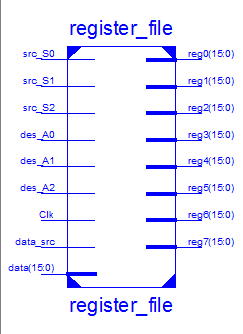
\includegraphics[height=3in]{reg.png}
\break
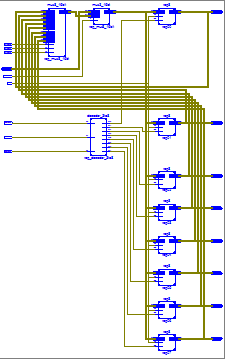
\includegraphics[height=3in]{all.png}
\end{align*}\\



\pagebreak
\subsection{REG8}\label{sec:result}

\begin{lstlisting}
library IEEE;
use IEEE.STD_LOGIC_1164.ALL;
use IEEE.STD_LOGIC_ARITH.ALL;
use IEEE.STD_LOGIC_UNSIGNED.ALL;
entity reg8 is
    Port ( load : in  STD_LOGIC;
           Clk : in  STD_LOGIC;
           D : in  STD_LOGIC_VECTOR(15 downto 0);
           Q : out  STD_LOGIC_VECTOR(15 downto 0));
end reg8;

architecture Behavioral of reg8 is

begin
process(Clk)
begin 
		if(rising_edge(Clk)) then 
			if(load ='1') then 
				Q<= D after 5ns;
			end if;
		end if;
	end process;
end Behavioral;
\end{lstlisting}

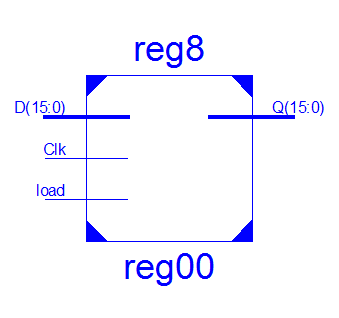
\includegraphics[width=6cm, height=8cm]{reg8.png}


\pagebreak
\subsection{DECODER}\label{sec:result}

\begin{lstlisting}
library IEEE;
use IEEE.STD_LOGIC_1164.ALL;
use IEEE.STD_LOGIC_ARITH.ALL;
use IEEE.STD_LOGIC_UNSIGNED.ALL;


entity decoder_3to8 is
    Port ( A0 : in  STD_LOGIC;
           A1 : in  STD_LOGIC;
           A2 : in  STD_LOGIC;
           Q0 : out  STD_LOGIC;
           Q1 : out  STD_LOGIC;
           Q2 : out  STD_LOGIC;
           Q3 : out  STD_LOGIC;
           Q4 : out  STD_LOGIC;
           Q5 : out  STD_LOGIC;
           Q6 : out  STD_LOGIC;
           Q7 : out  STD_LOGIC);
end decoder_3to8;

architecture Behavioral of decoder_3to8 is

begin
	Q0 <= ((	NOT A0) AND (NOT A1) AND (NOT A2)) AFTER 5ns;
	Q1 <= ((	NOT A0) AND (NOT A1) AND A2) AFTER 5ns;
	Q2 <= ((	NOT A0) AND A1 AND (NOT A2)) AFTER 5ns;
	Q3 <= ((	NOT A0) AND A1 AND A2) AFTER 5ns;
	Q4 <= (A0 AND (NOT A1) AND (NOT A2)) AFTER 5ns;
	Q5 <= (A0 AND (NOT A1) AND A2) AFTER 5ns;
	Q6 <= (A0 AND A1 AND (NOT A2)) AFTER 5ns;
	Q7 <= (A0 AND A1 AND A2) AFTER 5ns;


end Behavioral;
\end{lstlisting}

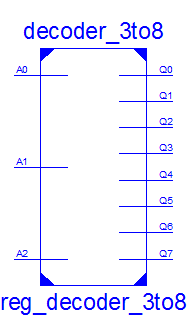
\includegraphics[width=5cm, height=7cm]{decoder.png}
\pagebreak
\subsection{MUX3}\label{sec:result}

\begin{lstlisting}

library IEEE;
use IEEE.STD_LOGIC_1164.ALL;
use IEEE.STD_LOGIC_ARITH.ALL;
use IEEE.STD_LOGIC_UNSIGNED.ALL;


entity mux3_16bit is
    Port ( s : in  STD_LOGIC;
           In0 : in  STD_LOGIC_VECTOR(15 downto 0);
           In1 : in  STD_LOGIC_VECTOR(15 downto 0);
           Z : out  STD_LOGIC_VECTOR(15 downto 0));
end mux3_16bit;

architecture Behavioral of mux3_16bit is

begin
	Z <= In0 after 5ns when s = '0' else
			In1 after 5ns when s = '1' else
			x"0000" after 5ns;

end Behavioral;
\end{lstlisting}

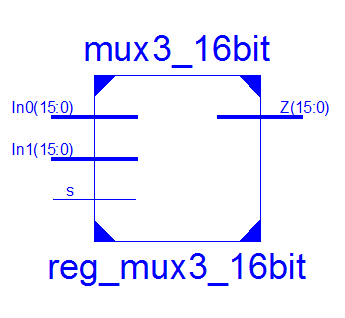
\includegraphics[width=6cm, height=8cm]{mux3.png}

\pagebreak
\subsection{MUX8}\label{sec:result}

\begin{lstlisting}

library IEEE;
use IEEE.STD_LOGIC_1164.ALL;
use IEEE.STD_LOGIC_ARITH.ALL;
use IEEE.STD_LOGIC_UNSIGNED.ALL;

entity mux8_16bit is
    Port ( S0 : in  STD_LOGIC;
           S1 : in  STD_LOGIC;
           S2 : in  STD_LOGIC;
           In0 : in  STD_LOGIC_VECTOR(15 downto 0);
           In1 : in  STD_LOGIC_VECTOR(15 downto 0);
           In2 : in  STD_LOGIC_VECTOR(15 downto 0);
           In3 : in  STD_LOGIC_VECTOR(15 downto 0);
           In4 : in  STD_LOGIC_VECTOR(15 downto 0);
           In5 : in  STD_LOGIC_VECTOR(15 downto 0);
           In6 : in  STD_LOGIC_VECTOR(15 downto 0);
           In7 : in  STD_LOGIC_VECTOR(15 downto 0);
           Z : out  STD_LOGIC_VECTOR(15 downto 0));
end mux8_16bit;

architecture Behavioral of mux8_16bit is

begin
	Z <= In0 after 5ns when S0 = '0' and S1 = '0' and S2 = '0' else 
			In1 after 5ns when S0 = '0' and S1 = '0' and S2 = '1' else 
			In2 after 5ns when S0 = '0' and S1 = '1' and S2 = '0' else 
			In3 after 5ns when S0 = '0' and S1 = '1' and S2 = '1' else
			In4 after 5ns when S0 = '1' and S1 = '0' and S2 = '0' else
			In5 after 5ns when S0 = '1' and S1 = '0' and S2 = '1' else
			In6 after 5ns when S0 = '1' and S1 = '1' and S2 = '0' else
			In7 after 5ns when S0 = '1' and S1 = '1' and S2 = '1' else
			x"0000" after 5ns;
end Behavioral;

\end{lstlisting}

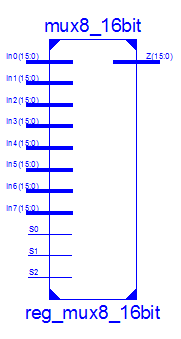
\includegraphics[width=5cm, height=7cm]{mux8.png}






\pagebreak

\section{TESTBENCHES}

\subsection{REGISTER FILE 1}\label{sec:result}

\begin{lstlisting}
LIBRARY ieee;
USE ieee.std_logic_1164.ALL;
 
-- Uncomment the following library declaration if using
-- arithmetic functions with Signed or Unsigned values
--USE ieee.numeric_std.ALL;
 
ENTITY test_register_file IS
END test_register_file;
 
ARCHITECTURE behavior OF test_register_file IS 
 
    -- Component Declaration for the Unit Under Test (UUT)
 
    COMPONENT register_file
    PORT(
         src_S0 : IN  std_logic;
         src_S1 : IN  std_logic;
         src_S2 : IN  std_logic;
         des_A0 : IN  std_logic;
         des_A1 : IN  std_logic;
         des_A2 : IN  std_logic;
         Clk : IN  std_logic;
         data_src : IN  std_logic;
         data : IN  std_logic_vector(15 downto 0);
         reg0 : OUT  std_logic_vector(15 downto 0);
         reg1 : OUT  std_logic_vector(15 downto 0);
         reg2 : OUT  std_logic_vector(15 downto 0);
         reg3 : OUT  std_logic_vector(15 downto 0);
         reg4 : OUT  std_logic_vector(15 downto 0);
         reg5 : OUT  std_logic_vector(15 downto 0);
         reg6 : OUT  std_logic_vector(15 downto 0);
         reg7 : OUT  std_logic_vector(15 downto 0)
        );
    END COMPONENT;
    

   --Inputs
   signal src_S0 : std_logic := '0';
   signal src_S1 : std_logic := '0';
   signal src_S2 : std_logic := '0';
   signal des_A0 : std_logic := '0';
   signal des_A1 : std_logic := '0';
   signal des_A2 : std_logic := '0';
   signal Clk : std_logic := '0';
   signal data_src : std_logic := '0';
   signal data : std_logic_vector(15 downto 0) := (others => '0');

 	--Outputs
   signal reg0 : std_logic_vector(15 downto 0);
   signal reg1 : std_logic_vector(15 downto 0);
   signal reg2 : std_logic_vector(15 downto 0);
   signal reg3 : std_logic_vector(15 downto 0);
   signal reg4 : std_logic_vector(15 downto 0);
   signal reg5 : std_logic_vector(15 downto 0);
   signal reg6 : std_logic_vector(15 downto 0);
   signal reg7 : std_logic_vector(15 downto 0);

   -- Clock period definitions
   constant Clk_period : time := 10 ns;
 
BEGIN
 
	-- Instantiate the Unit Under Test (UUT)
   uut: register_file PORT MAP (
          src_S0 => src_S0,
          src_S1 => src_S1,
          src_S2 => src_S2,
          des_A0 => des_A0,
          des_A1 => des_A1,
          des_A2 => des_A2,
          Clk => Clk,
          data_src => data_src,
          data => data,
          reg0 => reg0,
          reg1 => reg1,
          reg2 => reg2,
          reg3 => reg3,
          reg4 => reg4,
          reg5 => reg5,
          reg6 => reg6,
          reg7 => reg7
        );

   -- Clock process definitions
   Clk_process :process
   begin
		Clk <= '0';
		wait for Clk_period/2;
		Clk <= '1';
		wait for Clk_period/2;
   end process;
 

   -- Stimulus process
   stim_proc: process
   begin		
		wait for 10 ns;
			des_A0 <= '0';
			des_A1 <= '0';
			des_A2 <= '0';
			data <= x"FFFF";
		
		wait for 10 ns;
			des_A0 <= '0';
			des_A1 <= '0';
			des_A2 <= '1';
			data <= x"EEEE";
			
		wait for 10 ns;
			des_A0 <= '0';
			des_A1 <= '1';
			des_A2 <= '0';
			data <= x"DDDD";
		
		wait for 10 ns;
			des_A0 <= '0';
			des_A1 <= '1';
			des_A2 <= '1';
			data <= x"CCCC";
			
			wait for 10 ns;
			des_A0 <= '1';
			des_A1 <= '0';
			des_A2 <= '0';
			data <= x"BBBB";
		
		wait for 10 ns;
			des_A0 <= '1';
			des_A1 <= '0';
			des_A2 <= '1';
			data <= x"AAAA";
			
		wait for 10 ns;
			des_A0 <= '1';
			des_A1 <= '1';
			des_A2 <= '0';
			data <= x"9999";
		
		wait for 10 ns;
			des_A0 <= '1';
			des_A1 <= '1';
			des_A2 <= '1';
			data <= x"0000";
	  
    
   end process;

END;
\end{lstlisting}
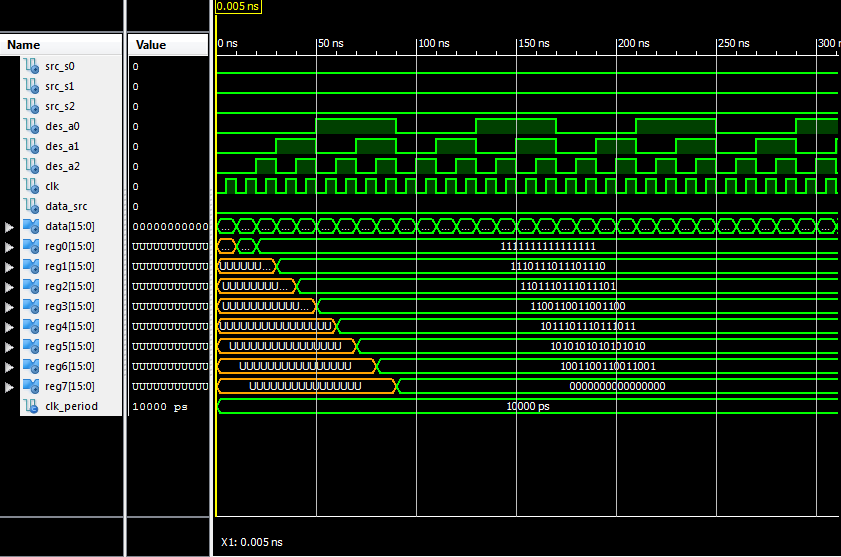
\includegraphics[width=10cm, height=5cm]{test_reg_file.png}

\pagebreak

\subsection{REGISTER FILE 2}\label{sec:result}

\begin{lstlisting}
LIBRARY ieee;
USE ieee.std_logic_1164.ALL;
 
-- Uncomment the following library declaration if using
-- arithmetic functions with Signed or Unsigned values
--USE ieee.numeric_std.ALL;
 
ENTITY test_register_file_2 IS
END test_register_file_2;
 
ARCHITECTURE behavior OF test_register_file_2 IS 
 
    -- Component Declaration for the Unit Under Test (UUT)
 
    COMPONENT register_file
    PORT(
         src_S0 : IN  std_logic;
         src_S1 : IN  std_logic;
         src_S2 : IN  std_logic;
         des_A0 : IN  std_logic;
         des_A1 : IN  std_logic;
         des_A2 : IN  std_logic;
         Clk : IN  std_logic;
         data_src : IN  std_logic;
         data : IN  std_logic_vector(15 downto 0);
         reg0 : OUT  std_logic_vector(15 downto 0);
         reg1 : OUT  std_logic_vector(15 downto 0);
         reg2 : OUT  std_logic_vector(15 downto 0);
         reg3 : OUT  std_logic_vector(15 downto 0);
         reg4 : OUT  std_logic_vector(15 downto 0);
         reg5 : OUT  std_logic_vector(15 downto 0);
         reg6 : OUT  std_logic_vector(15 downto 0);
         reg7 : OUT  std_logic_vector(15 downto 0)
        );
    END COMPONENT;
    

   --Inputs
   signal src_S0 : std_logic := '0';
   signal src_S1 : std_logic := '0';
   signal src_S2 : std_logic := '0';
   signal des_A0 : std_logic := '0';
   signal des_A1 : std_logic := '0';
   signal des_A2 : std_logic := '0';
   signal Clk : std_logic := '0';
   signal data_src : std_logic := '0';
   signal data : std_logic_vector(15 downto 0) := (others => '0');

 	--Outputs
   signal reg0 : std_logic_vector(15 downto 0);
   signal reg1 : std_logic_vector(15 downto 0);
   signal reg2 : std_logic_vector(15 downto 0);
   signal reg3 : std_logic_vector(15 downto 0);
   signal reg4 : std_logic_vector(15 downto 0);
   signal reg5 : std_logic_vector(15 downto 0);
   signal reg6 : std_logic_vector(15 downto 0);
   signal reg7 : std_logic_vector(15 downto 0);

   -- Clock period definitions
   constant Clk_period : time := 10 ns;
 
BEGIN
 
	-- Instantiate the Unit Under Test (UUT)
   uut: register_file PORT MAP (
          src_S0 => src_S0,
          src_S1 => src_S1,
          src_S2 => src_S2,
          des_A0 => des_A0,
          des_A1 => des_A1,
          des_A2 => des_A2,
          Clk => Clk,
          data_src => data_src,
          data => data,
          reg0 => reg0,
          reg1 => reg1,
          reg2 => reg2,
          reg3 => reg3,
          reg4 => reg4,
          reg5 => reg5,
          reg6 => reg6,
          reg7 => reg7
        );

   -- Clock process definitions
   Clk_process :process
   begin
		Clk <= '0';
		wait for Clk_period/2;
		Clk <= '1';
		wait for Clk_period/2;
   end process;
 

   -- Stimulus process
   stim_proc: process
   begin		
      

      wait for 10ns;
			data <= x"FFFF";
			des_A0 <= '0';
			des_A1 <= '0';
			des_A2 <= '0';
		
			src_S0 <= '0';
			src_S0 <= '0';
			src_S0 <= '0';
			
		wait for 20ns;
			data <= x"EEEE";
			des_A0 <= '0';
			des_A1 <= '0';
			des_A2 <= '1';
		
			src_S0 <= '0';
			src_S0 <= '0';
			src_S0 <= '1';
			
		wait for 30ns;
			data <= x"DDDD";
			des_A0 <= '0';
			des_A1 <= '1';
			des_A2 <= '0';
		
			src_S0 <= '0';
			src_S0 <= '1';
			src_S0 <= '0';
			
		wait for 40ns;
			data <= x"CCCC";
			des_A0 <= '0';
			des_A1 <= '1';
			des_A2 <= '1';
		
			src_S0 <= '0';
			src_S0 <= '1';
			src_S0 <= '1';
			
			
		 wait for 50ns;
			data <= x"BBBB";
			des_A0 <= '1';
			des_A1 <= '0';
			des_A2 <= '0';
		
			src_S0 <= '1';
			src_S0 <= '0';
			src_S0 <= '0';
			
		wait for 60ns;
			data <= x"AAAA";
			des_A0 <= '1';
			des_A1 <= '0';
			des_A2 <= '1';
		
			src_S0 <= '1';
			src_S0 <= '0';
			src_S0 <= '1';
			
		wait for 70ns;
			data <= x"9999";
			des_A0 <= '1';
			des_A1 <= '1';
			des_A2 <= '0';
		
			src_S0 <= '1';
			src_S0 <= '1';
			src_S0 <= '0';
			
		wait for 80ns;
			data <= x"0000";
			des_A0 <= '1';
			des_A1 <= '1';
			des_A2 <= '1';
		
			src_S0 <= '1';
			src_S0 <= '1';
			src_S0 <= '1';
			
   end process;

END;
\end{lstlisting}

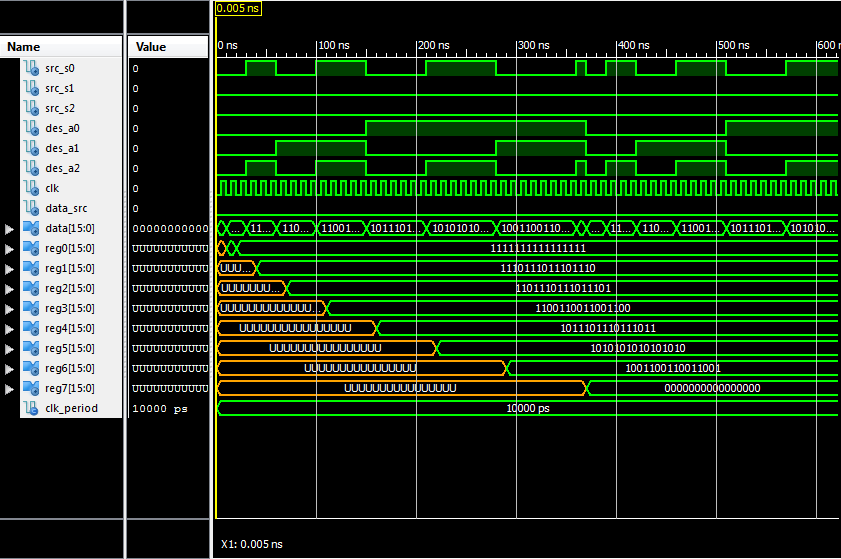
\includegraphics[width=16cm, height=8cm]{test_reg_file_2.png}
\pagebreak

\subsection{REG8}\label{sec:result}

\begin{lstlisting}
LIBRARY ieee;
USE ieee.std_logic_1164.ALL;
 

 
ENTITY test_reg8 IS
END test_reg8;
 
ARCHITECTURE behavior OF test_reg8 IS 
 
    -- Component Declaration for the Unit Under Test (UUT)
 
    COMPONENT reg8
    PORT(
         load : IN  std_logic;
         Clk : IN  std_logic;
         D : IN  std_logic_vector(15 downto 0);
         Q : OUT  std_logic_vector(15 downto 0)
        );
    END COMPONENT;
    

   --Inputs
   signal load : std_logic := '0';
   signal Clk : std_logic := '0';
   signal D : std_logic_vector(15 downto 0) := (others => '0');

 	--Outputs
   signal Q : std_logic_vector(15 downto 0);

   -- Clock period definitions
   constant Clk_period : time := 10 ns;
 
BEGIN
 
	-- Instantiate the Unit Under Test (UUT)
   uut: reg8 PORT MAP (
          load => load,
          Clk => Clk,
          D => D,
          Q => Q
        );

   -- Clock process definitions
   Clk_process :process
   begin
		Clk <= '0';
		wait for Clk_period/2;
		Clk <= '1';
		wait for Clk_period/2;
   end process;
 

   -- Stimulus process
   stim_proc: process
   begin		
	wait for 10ns;
	D <= x"FFFF";
	load <= '1';
	
	wait for 10ns;
	load <= '0';
	
	wait for 10ns;
	D<= x"AAAA";
	load <= '1';
	
      
   wait for 10ns;
	load <= '0';
	
   end process;
END;
\end{lstlisting}
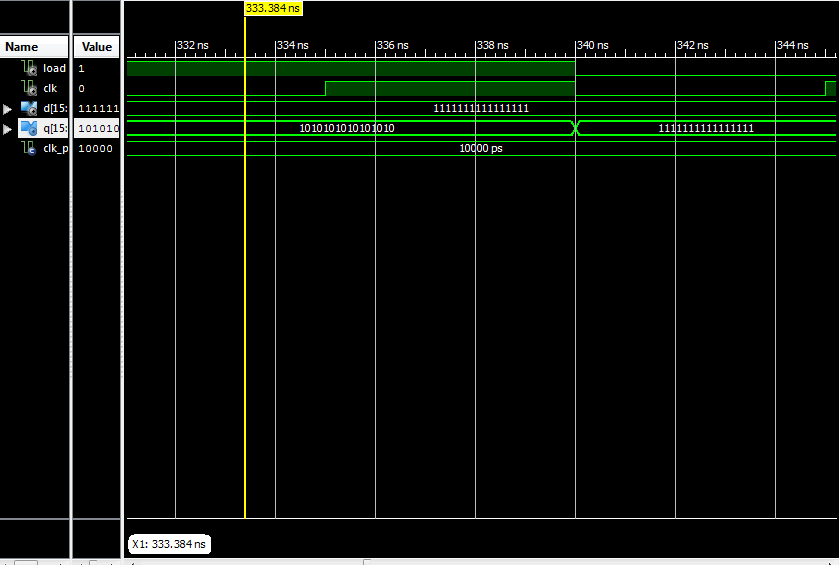
\includegraphics[width=16cm, height=8cm]{test_reg8.png}
\pagebreak
\subsection{DECODER}\label{sec:result}

\begin{lstlisting}
LIBRARY ieee;
USE ieee.std_logic_1164.ALL;
 
-- Uncomment the following library declaration if using
-- arithmetic functions with Signed or Unsigned values
--USE ieee.numeric_std.ALL;
 
ENTITY test_decoder_3to8 IS
END test_decoder_3to8;
 
ARCHITECTURE behavior OF test_decoder_3to8 IS 
 
    -- Component Declaration for the Unit Under Test (UUT)
 
    COMPONENT decoder_3to8
    PORT(
         A0 : IN  std_logic;
         A1 : IN  std_logic;
         A2 : IN  std_logic;
         Q0 : OUT  std_logic;
         Q1 : OUT  std_logic;
         Q2 : OUT  std_logic;
         Q3 : OUT  std_logic;
         Q4 : OUT  std_logic;
         Q5 : OUT  std_logic;
         Q6 : OUT  std_logic;
         Q7 : OUT  std_logic
        );
    END COMPONENT;
    

   --Inputs
   signal A0 : std_logic := '0';
   signal A1 : std_logic := '0';
   signal A2 : std_logic := '0';

 	--Outputs
   signal Q0 : std_logic;
   signal Q1 : std_logic;
   signal Q2 : std_logic;
   signal Q3 : std_logic;
   signal Q4 : std_logic;
   signal Q5 : std_logic;
   signal Q6 : std_logic;
   signal Q7 : std_logic;
   
BEGIN
 
	-- Instantiate the Unit Under Test (UUT)
   uut: decoder_3to8 PORT MAP (
          A0 => A0,
          A1 => A1,
          A2 => A2,
          Q0 => Q0,
          Q1 => Q1,
          Q2 => Q2,
          Q3 => Q3,
          Q4 => Q4,
          Q5 => Q5,
          Q6 => Q6,
          Q7 => Q7
        );

 
   -- Stimulus process
   stim_proc: process
   begin		
     wait for 10ns;
	  A0 <= '0';
	  A1 <= '0';
	  A2 <= '0';
	  
	  wait for 10ns;
	  A0 <= '0';
	  A1 <= '0';
	  A2 <= '1';
	  
	  wait for 10ns;
	  A0 <= '0';
	  A1 <= '1';
	  A2 <= '0';
	  
	  wait for 10ns;
	  A0 <= '0';
	  A1 <= '1';
	  A2 <= '1';

	  wait for 10ns;
	  A0 <= '1';
	  A1 <= '0';
	  A2 <= '0';
	  
	  wait for 10ns;
	  A0 <= '1';
	  A1 <= '0';
	  A2 <= '1';
	  
	  wait for 10ns;
	  A0 <= '1';
	  A1 <= '1';
	  A2 <= '0';
	  
	  wait for 10ns;
	  A0 <= '1';
	  A1 <= '1';
	  A2 <= '1';

   end process;

END;
\end{lstlisting}
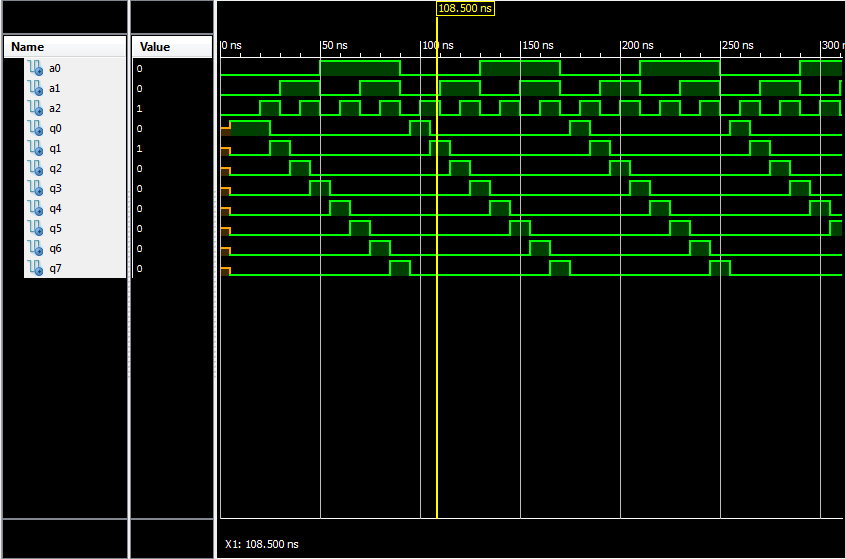
\includegraphics[width=16cm, height=8cm]{test_decoder.png}

\pagebreak

\subsection{MUX3}\label{sec:result}

\begin{lstlisting}
LIBRARY ieee;
USE ieee.std_logic_1164.ALL;
 

 
ENTITY test_mux3_16bit IS
END test_mux3_16bit;
 
ARCHITECTURE behavior OF test_mux3_16bit IS 
 
  
 
    COMPONENT mux3_16bit
    PORT(
         s : IN  std_logic;
         In0 : IN  std_logic_vector(15 downto 0);
         In1 : IN  std_logic_vector(15 downto 0);
         Z : OUT  std_logic_vector(15 downto 0)
        );
    END COMPONENT;
    

   --Inputs for the in0 and in1
   signal s : std_logic := '0';
   signal In0 : std_logic_vector(15 downto 0) := (others => '0');
   signal In1 : std_logic_vector(15 downto 0) := (others => '0');

 	--Outputs
   signal Z : std_logic_vector(15 downto 0);
   -- No clocks detected in port list. Replace <clock> below with 
   -- appropriate port name 
 
  
BEGIN
 
	-- Instantiate the Unit Under Test (UUT)
   uut: mux3_16bit PORT MAP (
          s => s,
          In0 => In0,
          In1 => In1,
          Z => Z
        );

   -- Signasl tested are here below
   stim_proc: process
   begin		
		wait for 10ns;
		In0<= x"FFFF";
		In1<= X"AAAA";
		
		wait for 10ns;
		s <= '1';
		
		wait for 10ns;
		s <= '0';
		
		wait for 10ns;
		s <= '0';
  
      wait;
   end process;

END;
\end{lstlisting}
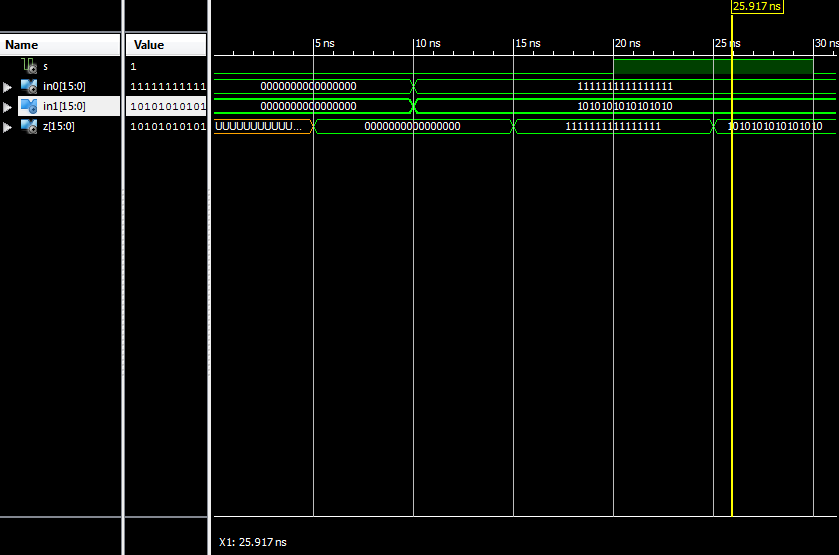
\includegraphics[width=16cm, height=8cm]{test_mux3.png}
\pagebreak

\subsection{MUX8}\label{sec:result}

\begin{lstlisting}
LIBRARY ieee;
USE ieee.std_logic_1164.ALL;
 
-- Uncomment the following library declaration if using
-- arithmetic functions with Signed or Unsigned values
--USE ieee.numeric_std.ALL;
 
ENTITY test_mux8_16bit IS
END test_mux8_16bit;
 
ARCHITECTURE behavior OF test_mux8_16bit IS 
 
    -- Component Declaration for the Unit Under Test (UUT)
 
    COMPONENT mux8_16bit
    PORT(
         S0 : IN  std_logic;
         S1 : IN  std_logic;
         S2 : IN  std_logic;
         In0 : IN  std_logic_vector(15 downto 0);
         In1 : IN  std_logic_vector(15 downto 0);
         In2 : IN  std_logic_vector(15 downto 0);
         In3 : IN  std_logic_vector(15 downto 0);
         In4 : IN  std_logic_vector(15 downto 0);
         In5 : IN  std_logic_vector(15 downto 0);
         In6 : IN  std_logic_vector(15 downto 0);
         In7 : IN  std_logic_vector(15 downto 0);
         Z : OUT  std_logic_vector(15 downto 0)
        );
    END COMPONENT;
    

   --Inputs
   signal S0 : std_logic := '0';
   signal S1 : std_logic := '0';
   signal S2 : std_logic := '0';
   signal In0 : std_logic_vector(15 downto 0) := (others => '0');
   signal In1 : std_logic_vector(15 downto 0) := (others => '0');
   signal In2 : std_logic_vector(15 downto 0) := (others => '0');
   signal In3 : std_logic_vector(15 downto 0) := (others => '0');
   signal In4 : std_logic_vector(15 downto 0) := (others => '0');
   signal In5 : std_logic_vector(15 downto 0) := (others => '0');
   signal In6 : std_logic_vector(15 downto 0) := (others => '0');
   signal In7 : std_logic_vector(15 downto 0) := (others => '0');

 	--Outputs
   signal Z : std_logic_vector(15 downto 0);
  
BEGIN
 
	-- Instantiate the Unit Under Test (UUT)
   uut: mux8_16bit PORT MAP (
          S0 => S0,
          S1 => S1,
          S2 => S2,
          In0 => In0,
          In1 => In1,
          In2 => In2,
          In3 => In3,
          In4 => In4,
          In5 => In5,
          In6 => In6,
          In7 => In7,
          Z => Z
        );

 
   -- Stimulus process
   stim_proc: process
   begin		
	
		In0 <= x"FFFF";
		In0 <= x"EEEE";
		In0 <= x"DDDD";
		In0 <= x"CCCC";
		In0 <= x"BBBB";
		In0 <= x"AAAA";
		In0 <= x"9999";
		In0 <= x"0000";
     
		wait for 10ns;
		S0 <= '0';
		S1 <= '0';
		S2 <= '0';
		
		wait for 10ns;
		S0 <= '0';
		S1 <= '0';
		S2 <= '1';
		
		wait for 10ns;
		S0 <= '0';
		S1 <= '1';
		S2 <= '0';
		
		wait for 10ns;
		S0 <= '0';
		S1 <= '1';
		S2 <= '1';
		
		wait for 10ns;
		S0 <= '1';
		S1 <= '0';
		S2 <= '0';
		
		wait for 10ns;
		S0 <= '1';
		S1 <= '0';
		S2 <= '1';
		
		wait for 10ns;
		S0 <= '1';
		S1 <= '1';
		S2 <= '0';
		
		wait for 10ns;
		S0 <= '1';
		S1 <= '1';
		S2 <= '1';
   end process;

END;
\end{lstlisting}
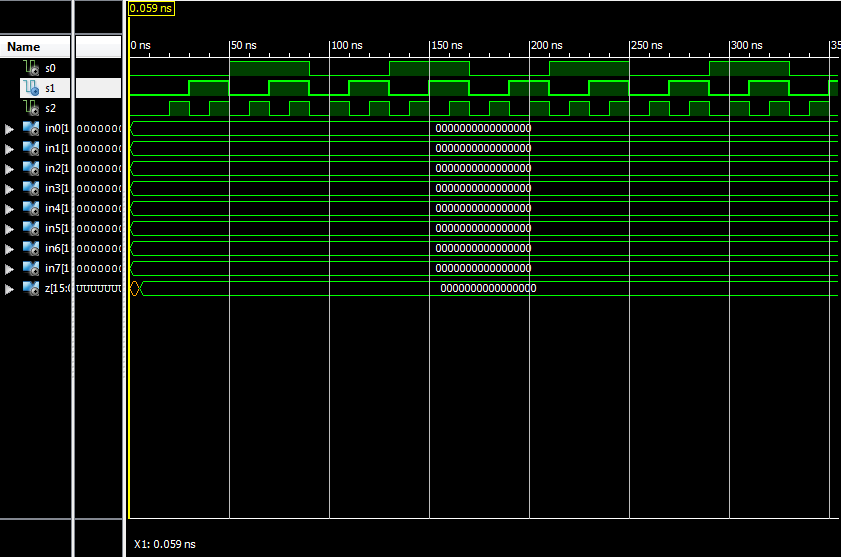
\includegraphics[width=16cm, height=8cm]{test_mux8.png}

	
\end{document}
